\chapter{Física sin miedo}

\begin{enpocas}
Vectores, las leyes de Newton aplicadas al dron, por qué el empuje crece con el cuadrado de la
velocidad, qué es la inercia, qué son los marcos de referencia (ENU, NED, cuerpo) y cómo se describe
una rotación. Al final, las ecuaciones del dron en una página.
\end{enpocas}

\section{Vectores}

Muchas cantidades físicas tienen tamaño y dirección: la velocidad del dron es ``3~m/s \emph{hacia el
este}''. Son \textbf{vectores} y se dibujan como flechas; en tres dimensiones tienen tres componentes,
$v = (v_x, v_y, v_z)$. Posición, velocidad, aceleración, fuerza y velocidad angular son vectores.

\section{Las leyes de Newton aplicadas al dron}

\begin{enumerate}
  \item \textbf{Inercia.} Un cuerpo sigue como está mientras nadie lo empuje: un dron que avanza y deja
        de inclinarse sigue avanzando un rato.
  \item \textbf{$F = ma$.} Para el dron,
        \begin{equation}
        m\,\ddot p = \underbrace{T\,R\,e_3}_{\text{empuje}} \;\underbrace{-\,mg\,e_3}_{\text{peso}} \;+\; \underbrace{d(t)}_{\text{viento}}
        \end{equation}
        con $T$ el empuje total, $R e_3$ la dirección ``arriba'' del dron (cambia si se inclina) y
        $e_3=(0,0,1)$.
  \item \textbf{Acción y reacción.} La hélice empuja aire hacia abajo y el aire la empuja hacia arriba;
        además, al girarla, el motor intenta girar al dron al revés (por eso las hélices van en pares que
        giran en sentidos opuestos).
\end{enumerate}

\section{Empuje: el cuadrado de la velocidad}

El empuje de una hélice es aproximadamente $f = k_f\,\omega^2$. En el Tarot 650, $k_f = 4.24\times
10^{-5}$~N/(rad/s)$^2$ y $\omega_{max} = 680$~rad/s, así que cada motor da hasta 19.6~N. Cada hélice
produce además un par de arrastre $k_m f$ ($k_m = 0.016$~m) que intenta girar al dron.

\begin{recuerda}
Los motores no cambian de velocidad al instante: en el Tarot simulado tienen constantes de tiempo de
0.03~s al acelerar y 0.05~s al frenar (en el x500, 12.5 y 25~ms). Ese retardo, aunque pequeño, limita qué tan agresivo puede ser el control.
\end{recuerda}

\section{Inercia de rotación y par}

Para girar importa el \textbf{momento de inercia} $J$: cuánto se resiste un cuerpo a cambiar su giro.
El Tarot 650 completo (con sus rotores) tiene 0.0341, 0.0361 y 0.0660~kg\,m$^2$ en sus tres ejes. Lo que hace girar es un \textbf{par}
$\tau$, una fuerza aplicada a cierta distancia del centro:
\begin{equation}
J\,\dot\omega = \tau - \omega\times J\omega .
\end{equation}

\begin{leccion}
Un detalle de menos de un milímetro tuvo efectos visibles. La cámara (50~g) tiene su centro de masa a
3~cm del eje y corre el del dron completo 0.7~mm en el x500, el vehículo de las primeras corridas
(0.67~mm en el Tarot). Eso produce un par pequeño pero constante que el controlador
neuronal original no sabía compensar: el dron se quedaba inclinado $\approx$1° y a $\approx$0.2~m del
punto deseado (capítulo~\ref{cap:control-neuronal}).
\end{leccion}

\section{Marcos de referencia: ¿desde dónde mido?}

\begin{description}
  \item[Mundo ENU] (Este, Norte, Arriba): fijo al suelo, con origen en el centro del bosque. Lo usan
        Gazebo y ROS.
  \item[Mundo NED] (Norte, Este, Abajo): el mismo lugar con otros ejes. Lo usan PX4 y ArduPilot.
  \item[Cuerpo:] pegado al dron. En ROS: FLU (frente, izquierda, arriba); en PX4: FRD (frente,
        derecha, abajo).
  \item[Cámara:] eje óptico hacia abajo, ``derecha'' y ``abajo'' de la imagen.
\end{description}

\begin{figure}[H]
\centering
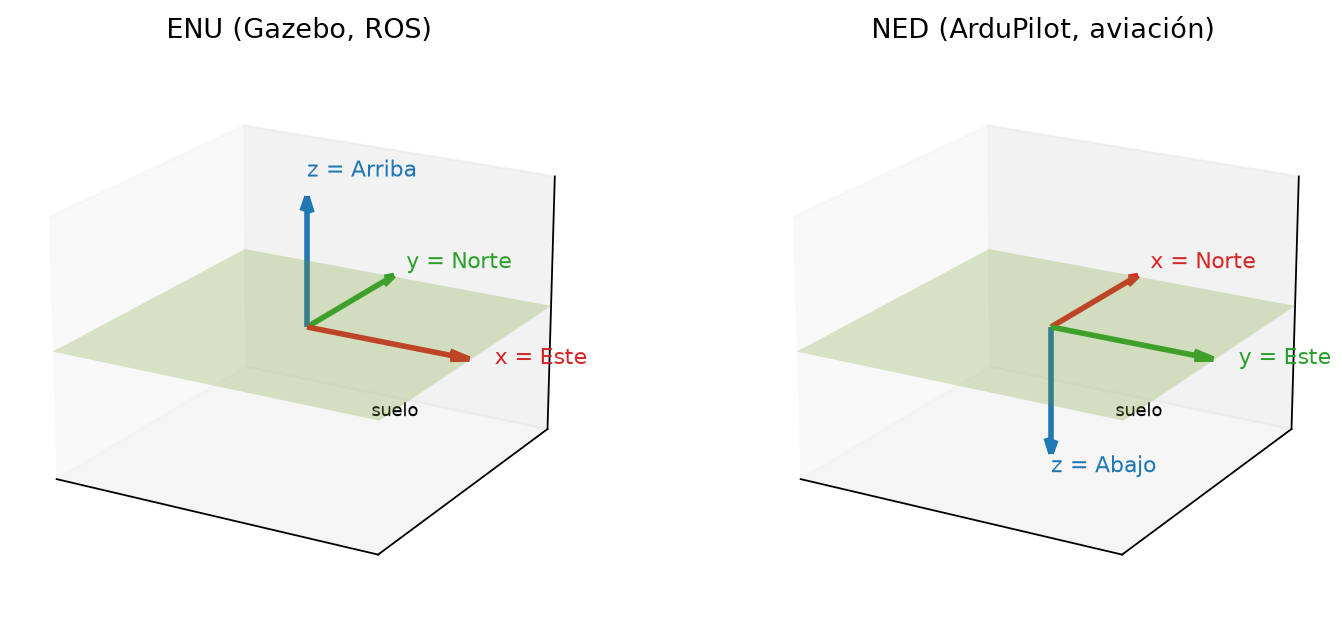
\includegraphics[width=0.9\textwidth]{c_marcos.png}
\caption{ENU y NED. Pasar de uno al otro es intercambiar $x$ con $y$ y cambiar el signo de $z$.}
\end{figure}

\begin{aviso}
Confundir marcos es la causa de error número uno en drones. En este proyecto conviven cinco (ENU, NED,
FLU, FRD y cámara). Cada conversión está en una función con nombre (\cod{ned_a_enu},
\cod{R_enu_flu}, \cod{R_BC}...) y probada en \cod{test/test_mision.py}.
\end{aviso}

\section{Rotaciones}

La orientación se describe con tres ángulos (alabeo $\phi$, cabeceo $\theta$, guiñada $\psi$) o con una
\textbf{matriz de rotación} $R$, cuyas columnas son los ejes del dron vistos desde el mundo; PX4 la
entrega como un \textbf{cuaternión} (cuatro números sin singularidades). En el localizador,
$R = R_z(\psi)R_y(\theta)R_x(\phi)$.

\begin{figure}[H]
\centering
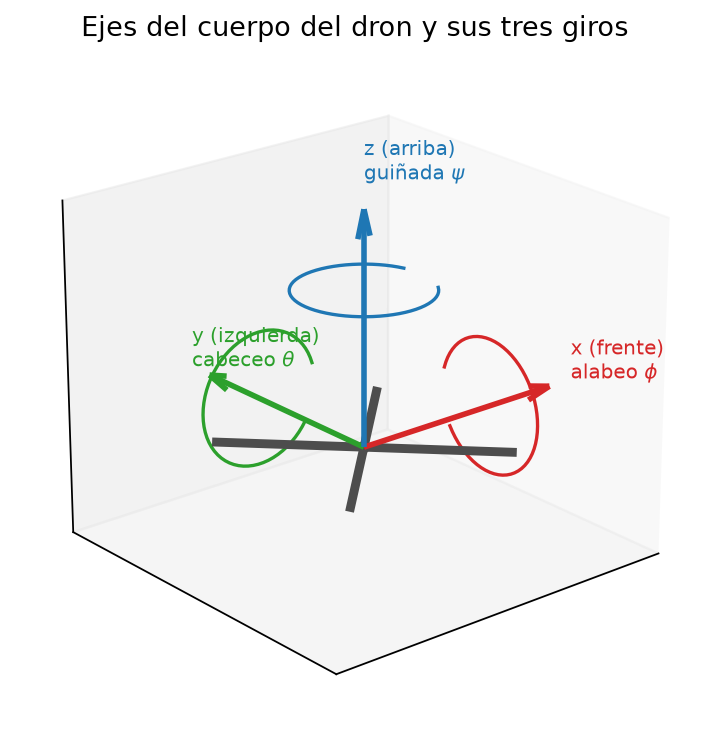
\includegraphics[width=0.55\textwidth]{c_ejes.png}
\caption{Ejes del cuerpo y sus tres giros.}
\end{figure}

\section{Las ecuaciones del dron en una página}

\begin{tcolorbox}[colback=white,colframe=NavyBlue!60!black,title=Modelo del cuadrirrotor]
\begin{align*}
\text{posición:}\quad & m\ddot p = T R e_3 - mg\,e_3 + d(t)\\
\text{orientación:}\quad & \dot R = R\hat\omega\\
\text{giro:}\quad & J\dot\omega = \tau - \omega\times J\omega\\
\text{motores:}\quad & f_i = k_f\omega_i^2,\quad \begin{bmatrix}T\\\tau\end{bmatrix} = A\,f,\quad
A = \begin{bmatrix}1&1&1&1\\ y_i & \cdots\\ -x_i & \cdots\\ -s_ik_m&\cdots\end{bmatrix}
\end{align*}
\end{tcolorbox}

\cod{codigo/sim_modelo.py} simula este modelo con el control base y reproduce las cifras del diseño
original del proyecto. Ese programa usa los parámetros del \textbf{x500} de PX4 (2.0~kg,
$k_f = 8.54858\times10^{-6}$, $\omega_{max} = 1000$~rad/s), no los del Tarot: las cifras y la figura
siguientes son del x500.

\begin{figure}[H]
\centering
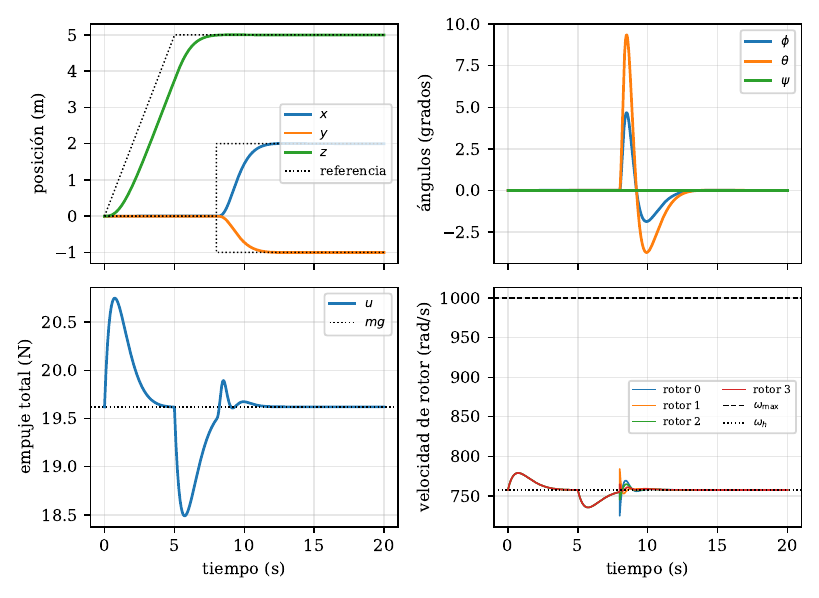
\includegraphics[width=0.85\textwidth]{manual_sim_modelo.png}
\caption{Salida de \cod{sim_modelo.py}: respuesta del modelo del x500 con el control base.}
\end{figure}
